\section{Mitigations Bypass}
\begin{frame}[fragile, allowframebreaks]{Mitigations Bypass}

	\begin{center}\huge
	Do these mitigations are enough??
	\end{center}
	
	\begin{block}{Spoiler: NO.}
	\begin{description}
	\item[ASLR bypass] via \emph{multiple input}, \emph{NOP sledge}, \emph{jmp2reg}, \emph{ROP} \ldots
	\item[DEP bypass] via \emph{ret2libc}, \emph{ROP} \ldots
	\item[Stack Cookie bypass] via Exception Handler exploiting (and other techniques which aren't treated here: eg. \emph{Heap-Overflow} \ldots)  
	\end{description}
	\end{block}
	
	\begin{center}
	\emph{This section aims to provide a quick overview on more advanced stack smashing.}
	\end{center}
	
\end{frame}

%%%%%%%%%%%%%%%%%%%%%%%%%%%%%%%%%%%%%%%%%%%%%%%%%%%%%%%%%%%%
\subsection{Multiple Input and Static Areas}
\begin{frame}[fragile, allowframebreaks]{Multiple Input and Static Areas}

	\begin{block}{Actually, not everything is randomized\ldots}
	Sections like .text or .bss (or some library memory space) are not randomized by ALSR.
	\end{block}
	
	\begin{block}{Expoit multiple input}
	\begin{list}{}{}
	\item If we can put our shellcode into a variable located in these memory areas (eg. \emph{global var}, \emph{static var}, \emph{environment}\ldots) then we should be able to correctly reference it.
	\item Enforcing this kind of attack often require to \emph{provide multiple inputs} (at least one in the stack and another in a not randomized place)
	\end{list}
	\end{block}
	
\end{frame}

%%%%%%%%%%%%%%%%%%%%%%%%%%%%%%%%%%%%%%%%%%%%%%%%%%%%%%%%%%%%
\subsection{NOP Sledge}
\begin{frame}[fragile, allowframebreaks]{NOP Sledge}
	
	\begin{block}{What if randomization is not truly random?}
	\begin{list}{-}{}
	\item In certain ALSR implementation (for several reasons) randomization 
		might present recurrent set of address.
	\item This enhance our chance to \emph{guess} the right address, but it's not enough
	\end{list}
	\end{block}
	
	\begin{block}{NOP sledge}
	\begin{list}{-}{}
		\item {\bf NOP} (0x90) is the \emph{No OPeration} instruction on x86 ISA
		\item Adding a long NOP prologue to our shellcode increase the valid address range usable to jump to our shellcode.
	\end{list}
	\end{block}

	\framebreak
	
	\begin{figure}
        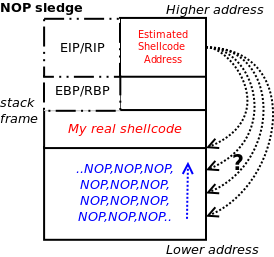
\includegraphics[width=0.6\textwidth]{imgs/nop-sledge.png}
        \label{fig:nop-sledge}
        \caption{NOP Sledge role during stack smashing}
    \end{figure}	
	
\end{frame}

%%%%%%%%%%%%%%%%%%%%%%%%%%%%%%%%%%%%%%%%%%%%%%%%%%%%%%%%%%%%
\subsection{JMP2Register}
\begin{frame}[fragile, allowframebreaks]{JMP2Register}

	\begin{block}{Changing scenario}
	\begin{list}{-}{}
	\item No static memory location
	\item No time to try to guess addresses
	\end{list}
	Try to think at how variables are referenced in Assembly\ldots
	\emph{Var. address could be stored in a register}
	\end{block}
	
	\framebreak
	
	\begin{figure}
        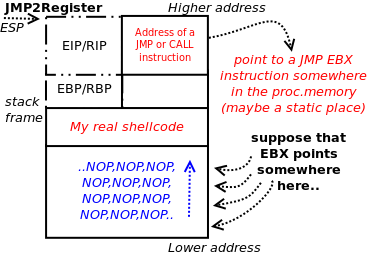
\includegraphics[width=0.65\textwidth]{imgs/jmp2reg.png}
        \label{fig:jmp2reg}
        \caption{Jmp2reg example with EBX register that contains an address of a stack memory location ({\bf area under attacker control})}
    \end{figure}	
	
	\framebreak
	
	\begin{block}{What If no jmp reg ?}
	Same trick could be exploited with other statements:
	\begin{itemize}
	\item \emph{call reg}
	\item \emph{push reg; ret}
	\item \emph{jmp [reg + offset]}
	\item \emph{pop; ret} if desired address lay on stack (\emph{pop;pop;ret} \emph{pop;pop;pop;ret} and so on)
	\end{itemize}
	\end{block}
	
\end{frame}

%%%%%%%%%%%%%%%%%%%%%%%%%%%%%%%%%%%%%%%%%%%%%%%%%%%%%%%%%%%%
\subsection{Exception Handler}
\begin{frame}[fragile, allowframebreaks]{Exception Handler}

\begin{itemize}
\item As seen before some stack protection check if the stack as been smashed before function return. So classic ``\emph{overwrite EBP+4}'' does not work.
\item Many languages support custom {\bf exception handling} statement (eg.C++)
\item \emph{May we execute our shellcode instead of user defined handler?}
\end{itemize}

\begin{block}{SEH based stack smashing}
Generally depends on how compiler handle user define Exception Handlers, and in many case its possible (with gcc and VC++ both).\\
{\bf Here we introduce how to exploit the VC++ SEH (Structured Exception Handler)}
\end{block}

\framebreak
	\begin{figure}
        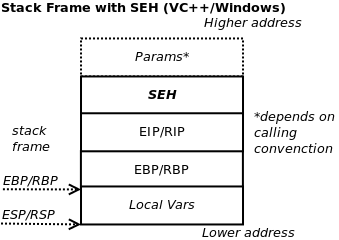
\includegraphics[width=0.65\textwidth]{imgs/seh-stack-frame.png}
        \label{fig:seh-stack-frame}
        \caption{Stack frame with SEH under Windows}
    \end{figure}	
\framebreak
	\begin{figure}
        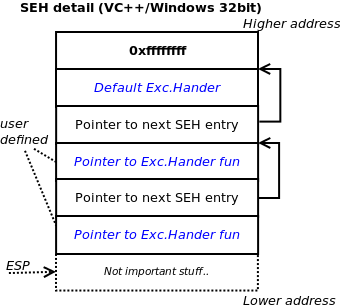
\includegraphics[width=0.55\textwidth]{imgs/seh-detail.png}
        \label{fig:seh-detail}
        \caption{SEH structure (list) under Windows}
    \end{figure}
   
\framebreak
	\begin{figure}
        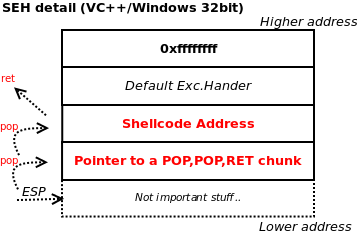
\includegraphics[width=0.6\textwidth]{imgs/seh-exploit.png}
        \label{fig:seh-exploit}
        \caption{SEH exploiting under Windows}
    \end{figure}

\end{frame}

%%%%%%%%%%%%%%%%%%%%%%%%%%%%%%%%%%%%%%%%%%%%%%%%%%%%%%%%%%%%
\subsection{Ret2libc}
\begin{frame}[fragile, allowframebreaks]{Ret2libc}

\begin{itemize}
\item Now we want to deal with {\bf DEP} countermeasure.
\item As you know no bytes in .data .stack .bss segments can be executed.
\end{itemize}

\begin{block}{What about executing some library code?}
\emph{libc} function \emph{system(char*cmd)} executes the command specified by the string pointed by its parameter. \\
May we craft the stack in a manner to simulate a function call without CALL?
\end{block}

\framebreak
	\begin{figure}
        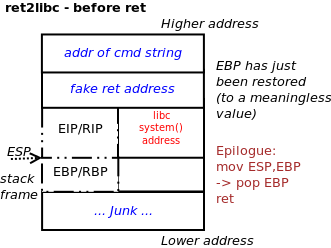
\includegraphics[width=0.65\textwidth]{imgs/ret2libc-1.png}
        \label{fig:ret2libc-1}
        \caption{Ret2libc fashioned stack smashing, before ret (stdcall ia32)}
    \end{figure}	
\framebreak
	\begin{figure}
        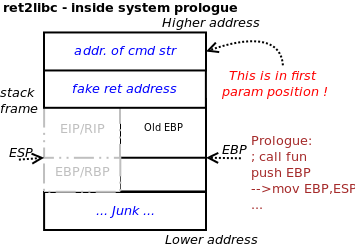
\includegraphics[width=0.65\textwidth]{imgs/ret2libc-2.png}
        \label{fig:ret2libc-2}
        \caption{Ret2libc fashioned stack smashing, executing target function prologue (stdcall ia32)}
    \end{figure}

\end{frame}

%%%%%%%%%%%%%%%%%%%%%%%%%%%%%%%%%%%%%%%%%%%%%%%%%%%%%%%%%%%%
\subsection{ROP}
\begin{frame}[fragile, allowframebreaks]{Return Oriented Programming}
	TBD
\end{frame}
